% !TeX root = ../main.tex

\chapter{面向性能预测的着色器性能数据集}

{\added 本章提出了面向性能预测的着色器性能数据集。渲染中的着色器程序的性能收集和理解面临多种挑战,本章的引言部分将首先介绍数据集工作面临的问题。之后,本章将详细介绍着色器收集和性能测量部分的实现。同时,为了更好的了解着色器程序本身的功能类型特征,本章同时将介绍一种使用基座语言模型来进行着色器类型标注的相关尝试。最后,本章将通过实验和分析验证本章提出的数据集的质量和分布信息。}

\section{引言}

{\added 着色器程序是利用 GPU 进行实时渲染的过程中,嵌入到渲染流水线中的程序片段。由于性能对于游戏等实时渲染程序来说至关重要,故而了解着色器程序的性能对于程序的优化来说可以起到一定的帮助。对于数据驱动的着色器程序性能预测方法来说,高质量的着色器程序性能数据是其成功的关键。同时,不同类型的着色器程序可能在不同平台上体现不同的性能特征,这些行为也需要跨越不同平台的着色器性能数据集加以刻画。然而,构建这样的数据集面临着如下挑战。

{\bf 其一},尚无用于着色器程序性能理解和学习的公开着色器性能数据集。经典的程序语言理解数据集,如其中包含 POJ-104 \cite{10.5555/3015812.3016002}、GitHub Java Corpus 等的 CodeXGLUE 数据集\cite{DBLP:journals/corr/abs-2102-04664},更多关注于代码的通用语义理解,而对性能部分关注较少。GPU 上的数据集,如 OpenCL 异构映射任务数据集\cite{8091247},则多只关注于通用计算方面,且程序的规模和丰富程度均需要进一步增强。

% TODO: 如果第二章基础知识部分增加了相关的说明,可以挪动到这里。
{\bf 其二},着色器程序的性能受到多种波动的影响,而现有的程序理解数据集中,多只有简单的运行时间,缺乏对于运行时间的稳定度的分析。例如,面向机器学习的大规模程序理解数据集 CodeNet \cite{DBLP:journals/corr/abs-2105-12655} 中,关于程序性能的标注只有 CPU 运行时间和运行内存两项。对于 GPU 上运行的程序来说,整个计算过程经过的环节更多,所以运行时间的不确定性也会更强。

{\bf 其三},着色器程序实现的效果多种多样,而程序的类型对于后续的理解工作会起到一定作用。例如,仅仅在片段着色器程序中,程序开发者就可以实现图 \ref{fig:shadertoy_gallery_ch3} 中多样的画面效果。程序开发者通常会在代码内和平台上留有一定程度的作品标签信息,如本章使用的数据来源 Shadertoy 平台就提供向上传作品的属性信息中添加 tag 的功能。然而,许多上传的着色器程序,其标注并不完备。

\begin{figure}[htbp]
  \centering
  \begin{minipage}[b]{\textwidth}
      \begin{subfigure}[b]{0.48\textwidth}
          
\includegraphics[width=\textwidth]{figures/shadertoy_cloud.png}
          \caption{过程化纹理生成 (PTG)}
          \label{fig:sub_textgen}
      \end{subfigure}
      \hfill % Adds horizontal space between the subfigures
      \begin{subfigure}[b]{0.48\textwidth}
          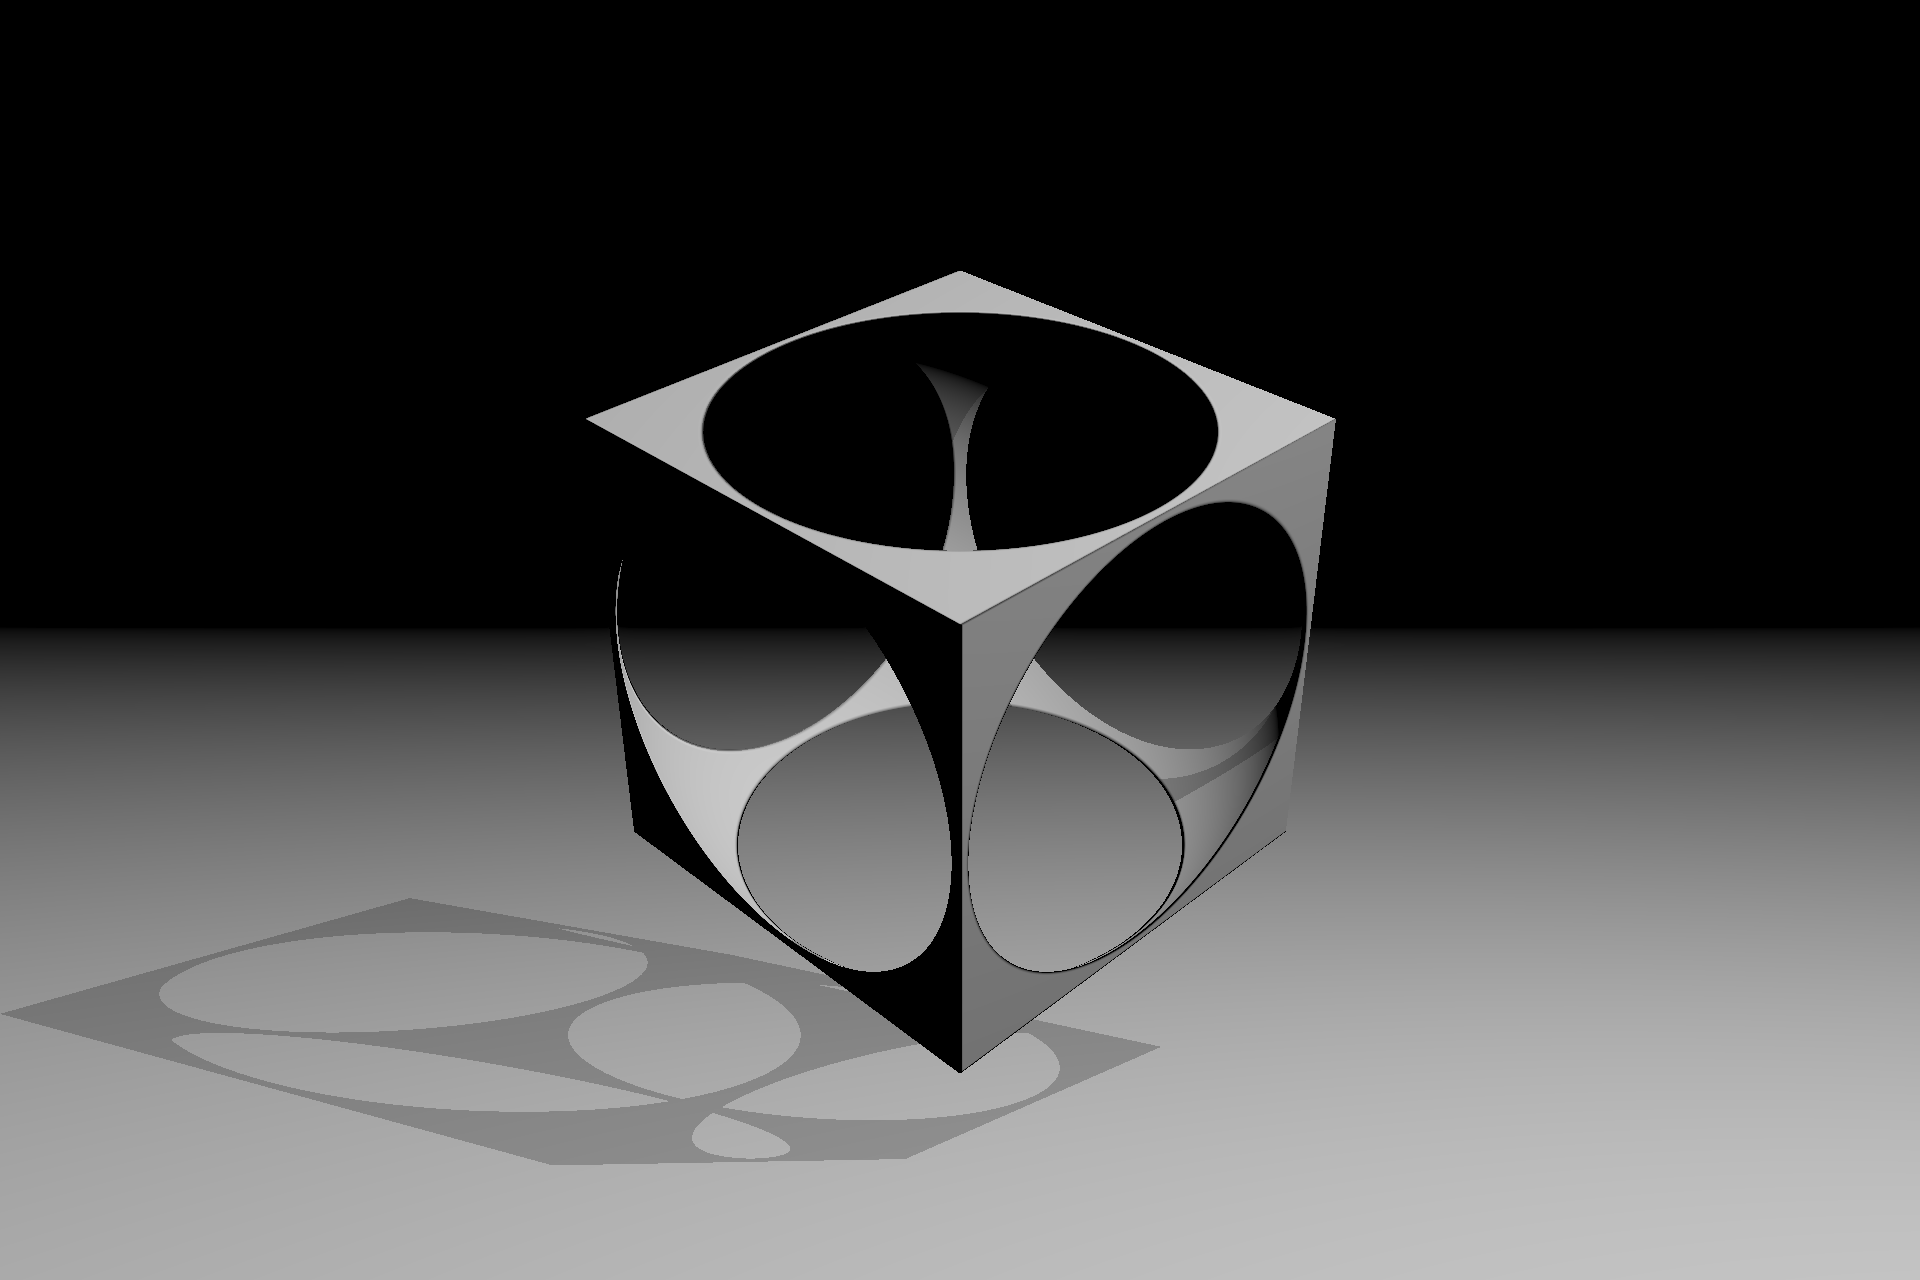
\includegraphics[width=\textwidth]{figures/shadertoy_csg.png}
          \caption{构造实体几何 (CSG)}
          \label{fig:sub_csg}
      \end{subfigure}
  \end{minipage}
  
  %\vspace{1em} % Adds vertical space between the rows of subfigures
  
  \begin{minipage}[b]{\textwidth}
      \begin{subfigure}[b]{0.48\textwidth}
          
\includegraphics[width=\textwidth]{figures/shadertoy_raymarching.png}
          \caption{光线步进 (Ray Marching)}
          \label{fig:sub_raymarching}
      \end{subfigure}
      \hfill % Adds horizontal space between the subfigures
      \begin{subfigure}[b]{0.48\textwidth}
          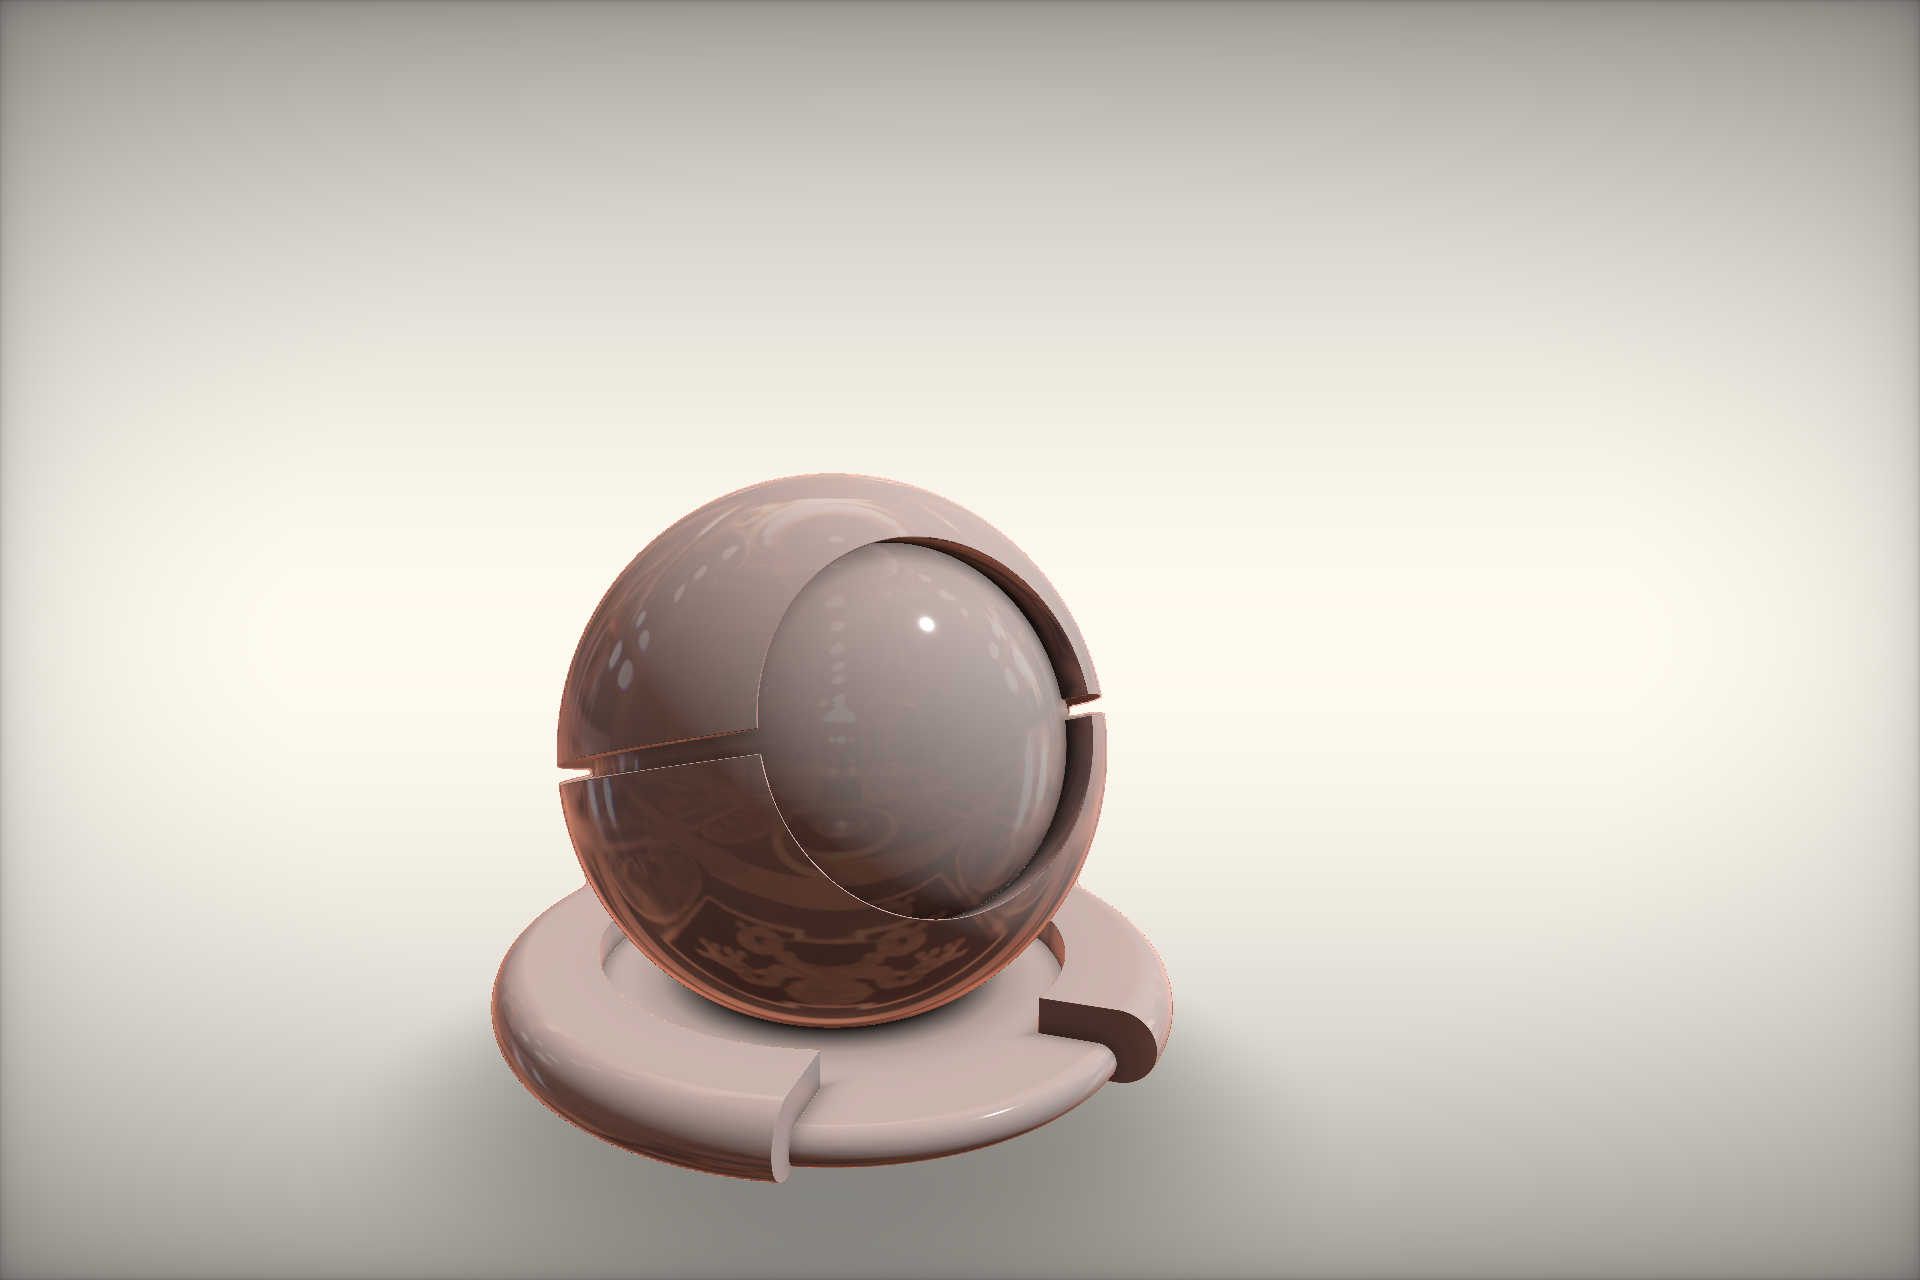
\includegraphics[width=\textwidth]{figures/shadertoy_pbr.png}
          \caption{基于物理的着色 (PBS)}
          \label{fig:sub_pbs}
      \end{subfigure}
  \end{minipage}
  
  \caption{Shadertoy 用户\cite{ShdrToyUser1, ShdrToyUser2}着色器程序效果示例与其使用的主要技术}
  \label{fig:shadertoy_gallery_ch3}
\end{figure}


本章提出的数据集将基本解决上述问题。针对问题一,本章所描述的方法构造了新的着色器性能数据集,其包含 5 个 GPU 平台,共 54667 个片段着色器性能样本。针对问题二,本章性能测量时使用了重复采样和 GPU 端时间戳测量,并在实验时对样本的变异系数进行了分析。针对问题三,本章探索了利用基座语言模型、结合人工进行半自动着色器类型标注的相关方法,为着色器数据集内的功能类型提供了参考。同时,本章提出的数据集将进一步给出在不同平台间有显著性能相对差异的着色器样本集合。并在实验部分给出数据集的质量评估。
}

\section{着色器收集和性能测量}

{\added 本章提出的数据集的数据来源于 Shadertoy\cite{Shadertoy} 网站上用户上传的着色器程序数据。} Shadertoy 是一个在线{\added 的着色器共享}平台,{\amend 其}允许用户创建、分享和查看着色器程序{\amend 并在线查看}渲染结果。

{\added 对于 GPU 上基于光栅化的图形渲染程序来说,其通常需要}指定管线的顶点和三角面索引输入,同时给出过程中用到的顶点、片元等着色器{\amend 以调用 GPU 进行绘制操作。}不过,出于降低上手门槛、让用户专注于创造新奇有趣的视觉效果本身的考虑,Shadertoy 平台上在进行显示绘制时,均{\amend 使用输入图元为覆盖全视口的两个三角形作为输入,且使用一个在顶点变换阶段原样输出的顶点着色器。}{\added 该着色器可以使用 WebGL Inspector \cite{WebGLInspector} 截出。}

作为示例,一个简单的 Shadertoy 着色器如图 \ref{fig:example_glsl_shadertoy_code_ch3} 中代码所示,其渲染结果如图 \ref{fig:example_shadertoy_output} 所示。

\begin{figure}  % 'h' for here, 't' for top, 'b' for bottom, 'p' for on a separate page
\centering

\begin{lstlisting}[language=GLSL]
void mainImage( out vec4 fragColor, in vec2 fragCoord )
{
    // 从 0 到 1 的归一化屏幕坐标
    vec2 uv = fragCoord/iResolution.xy;

    // 生成随时间 iTime 变化的像素颜色
    vec3 col = 0.5 + 0.5*cos(iTime+uv.xyx+vec3(0,1,5));

    // 输出到屏幕
    fragColor = vec4(col,1.0);
}
\end{lstlisting}
\caption{在屏幕上产生渐变颜色的 Shadertoy 代码示例}
\label{fig:example_glsl_shadertoy_code_ch3}
\end{figure}

\begin{figure}
  \centering
  
\includegraphics[width=0.65\textwidth]{figures/example_shadertoy_output.png}
  \caption{在屏幕上产生渐变颜色的 Shadertoy 效果示例}
  \label{fig:example_shadertoy_output_ch3}
\end{figure}

如图 \ref{fig:shadertoy_gallery_ch3},尽管在渲染时缺乏多样的几何输入,{\amend Shadertoy 上的着色器程序}仍然可以通过应用如光线步进(Ray Marching)\cite{Hart1996}, 过程化内容生成(Procedural Content Generation)等技术来创建能够产生复杂视觉效果的着色器。Shadertoy 网站收集的着色器在渲染技术方面覆盖相当完备{\amend,GPU 负载情况变化多样},故而{\amend 本章}以 Shadertoy 上的着色器为基础,构建片元着色器性能数据集。

\subsection{数据收集}

为了方便第三方程序的编写,Shadertoy 网站提供了基于 HTTP GET 的 API 接口,这为{\amend 数据集的}数据收集工作提供了一定便利。利用 Shadertoy API 进行数据收集的步骤大大致如下:

\begin{enumerate}
    \item 在 Shadertoy 网站上申请 API Key,从而得到 6 位的 API Key
    \item 请求 API,以得到所有用户上传的着色器的 ID
    \item 对每个 ID,请求 API 以得到 JSON 格式存储的着色器
\end{enumerate}

{\added Shadertoy 为了功能的丰富,其在网站功能上加入了简单的多遍渲染(Multi-pass Rendering)功能。所谓多遍渲染,即为多次调用绘制流水线,每次采用不同的着色器程序输入和最终的输出对象,并在最后的绘制流水线调用中进行合成。然而,通常可以认为,着色器性能的刻画,主要可以参考一次绘制流水线调用的耗时。故而,需要对 Shadertoy 中的着色器进行过滤和筛选,以获得需要的单遍渲染使用的着色器程序。}

Shadertoy 使用渲染通道(Render Pass)来刻画多遍渲染需要的信息。在其 JSON 格式存储的着色器的每个渲染通道内,存放有大致对应着一次绘制流水线绘制需要的纹理、Uniform 变量输入和着色器程序资源信息。同时,渲染通道之间的先后顺序为预先定义的顺序。基于对所爬取的着色器的观察,常见的渲染通道主要有 Image,Common 和 Buffer 三类。

{\bf Image 通道}是负责输出最终显示内容的渲染通道,是必须存在的。多数 Shadertoy 着色器程序只拥有 Image 通道。{\bf Common 通道}不是真正的渲染通道,而是作为例程代码,插入到所有其他渲染通道的着色器中。其用于定义多个渲染通道共享的、可重复使用的函数例程,而不直接输出内容,也不是必须存在的。{\bf Buffer 通道}则是用于记录程序状态或构建复杂图像效果的中间渲染通道,输出对象是专门的图像缓冲。其通常存储和操作着色器程序的中间数据,不是必须存在的通道。

对于 Shadertoy 的着色器程序来说,可以认为使用了 Buffer 通道的程序为多渲染通道程序,而只使用 Image 和 Common 通道的程序为单渲染通道程序。由于多渲染通道的程序可以认为是多个独立的单渲染通道程序的叠加,故而{\amend 数据集构建}时只着眼于处理单渲染通道的着色器程序。

{\added 在收集和过滤好单渲染通道的 Shadertoy 着色器程序,并将 Image 和 Common 通道的着色器代码进行合并,后就得到了可以被第 \ref{sec:perf_data_generation} 节将提出的性能数据生成环节使用的着色器程序。}
% Todo: 过滤后的信息可以参见实验部分的表

\subsection{性能数据生成}
\label{sec:perf_data_generation}

% TODO: amend from here

Shadertoy 上的着色器程序运行时需要在每帧提供一些预先设置好的 Uniform 变量资源。这些 Uniform 变量作为输入,其本身可以以 GLSL 的匿名 Uniform 块的形式被源码所引用,且可以大致分为屏幕数据、用户输入、时间和其它通道输入采样四种类别。例如,图 \ref{fig:example_glsl_shadertoy_code} 就使用了 iResolution 和 iTime 两个 Uniform 变量。一些常用的 Uniform 输入包括:
\begin{itemize}
    \item iTime: 当前的渲染时间
    \item iFrame: 当前渲染的帧编号
    \item iResolution: 当前的屏幕分辨率
    \item iMouse: 鼠标位置
    \item iDate: 年月日和时间信息
\end{itemize}

许多 Shadertoy 程序对上述输入进行更改的情况下,会产生出不同的画面。同时,Shadertoy 着色器程序的入口点函数 mainImage 与通常的片元着色器入口点函数不同。在 Shadertoy 网站上,用户上传的编译器会被拼接为 WebGL 可以执行的 OpenGL ES 着色器程序,并由浏览器的 WebGL 实现运行。

\section{着色器类型标注}


\section{实验和分析}


